\documentclass{article}
\usepackage{amsmath,amsthm,amssymb,amsfonts}
\usepackage{setspace,enumitem}
\usepackage{graphicx}
\usepackage{hyperref}
\usepackage{natbib}
\usepackage{afterpage}
\usepackage{xcolor}
\usepackage{etoolbox}
\usepackage{booktabs}
\usepackage{pdfpages}
\usepackage{multicol}
\usepackage{geometry}
\usepackage{accents}
\usepackage{bbm}
\hypersetup{
	colorlinks,
	linkcolor={blue!90!black},
	citecolor={red!90!black},
	urlcolor={blue!90!black}
}

\newtheorem{theorem}{Theorem}
\newtheorem{assumption}{Assumption}
\newtheorem{definition}{Definition}
\newtheorem{lemma}{Lemma}
\setlength{\parindent}{0cm}
\geometry{margin = 1in}

\newcommand{\R}{\mathbb{R}}
\newcommand{\ubar}[1]{\underaccent{\bar}{#1}}
\newcommand{\Int}{\text{Int}}
\newcommand{\xbf}{\mathbf{x}}
\newcommand{\Abf}{\mathbf{A}}
\newcommand{\Bbf}{\mathbf{B}}
\newcommand{\Gbf}{\mathbf{G}}
\newcommand{\bbf}{\mathbf{b}}
\newcommand{\one}{\mathbbm{1}}

\newtoggle{extended}
\settoggle{extended}{false}

\title{FIN 971A: Homework 1}
\author{Alex von Hafften }

\begin{document}

\maketitle

\section{Question 1}

\section{Question 2}

\begin{tabular}{lcccccc} \hline
 & (1) & (2) & (3) & (4) & (5) & (6) \\
VARIABLES & b\_lev\_tr & b\_lev\_tr & b\_lev\_tr & m\_lev\_tr & m\_lev\_tr & m\_lev\_tr \\ \hline
 &  &  &  &  &  &  \\
zee\_i\_b\_lev & 0.0274 & 0.0227 & 0.0180 &  &  &  \\
 & (0.0242) & (0.0198) & (0.0167) &  &  &  \\
zee\_l\_sales\_tr &  & 0.0189*** & 0.0257*** &  & 0.0248*** & 0.0351*** \\
 &  & (0.00166) & (0.00175) &  & (0.00175) & (0.00184) \\
zee\_m\_b\_tr &  & -0.0304*** & -0.0174*** &  & -0.0830*** & -0.0743*** \\
 &  & (0.00149) & (0.00130) &  & (0.00155) & (0.00148) \\
zee\_profit\_tr &  & -0.0341*** & -0.0396*** &  & -0.0536*** & -0.0596*** \\
 &  & (0.00135) & (0.00134) &  & (0.00142) & (0.00140) \\
zee\_tang\_tr &  & 0.0525*** & 0.0314*** &  & 0.0353*** & 0.0206*** \\
 &  & (0.00197) & (0.00181) &  & (0.00175) & (0.00180) \\
zee\_ind\_b\_lev &  &  & 0.0590*** &  &  & 0.0453*** \\
 &  &  & (0.00208) &  &  & (0.00164) \\
zee\_cf\_vol\_tr &  &  & -0.0132*** &  &  & -0.0166*** \\
 &  &  & (0.00123) &  &  & (0.00121) \\
pays\_dv &  &  & -0.0601*** &  &  & -0.0759*** \\
 &  &  & (0.00301) &  &  & (0.00330) \\
zee\_i\_m\_lev &  &  &  & 0.134*** & 0.102*** & 0.0922*** \\
 &  &  &  & (0.00225) & (0.00219) & (0.00212) \\
Constant & 0.254*** & 0.244*** & 0.282*** & 0.298*** & 0.285*** & 0.329*** \\
 & (0.00167) & (0.00160) & (0.00208) & (0.00195) & (0.00169) & (0.00226) \\
 &  &  &  &  &  &  \\
Observations & 106,957 & 106,957 & 106,957 & 94,490 & 94,490 & 94,490 \\
 R-squared & 0.021 & 0.148 & 0.226 & 0.259 & 0.428 & 0.465 \\ \hline
\multicolumn{7}{c}{ Robust standard errors in parentheses} \\
\multicolumn{7}{c}{ *** p$<$0.01, ** p$<$0.05, * p$<$0.1} \\
\end{tabular}



\begin{tabular}{lcccccc} \hline
 & (1) & (2) & (3) & (4) & (5) & (6) \\
VARIABLES & b\_lev\_tr & b\_lev\_tr & b\_lev\_tr & m\_lev\_tr & m\_lev\_tr & m\_lev\_tr \\ \hline
 &  &  &  &  &  &  \\
zee\_i\_b\_lev & 0.296*** & 0.246*** & 0.211*** &  &  &  \\
 & (0.0133) & (0.0128) & (0.0123) &  &  &  \\
zee\_l\_sales\_tr &  & 0.0192*** & 0.0264*** &  & 0.0334*** & 0.0422*** \\
 &  & (0.00229) & (0.00246) &  & (0.00290) & (0.00307) \\
zee\_m\_b\_tr &  & -0.0141*** & -0.00902*** &  & -0.0887*** & -0.0813*** \\
 &  & (0.00266) & (0.00264) &  & (0.00364) & (0.00347) \\
zee\_profit\_tr &  & -0.0630*** & -0.0578*** &  & -0.108*** & -0.103*** \\
 &  & (0.00329) & (0.00314) &  & (0.00433) & (0.00386) \\
zee\_tang\_tr &  & 0.0350*** & 0.0203*** &  & 0.0389*** & 0.0185*** \\
 &  & (0.00250) & (0.00261) &  & (0.00299) & (0.00316) \\
zee\_ind\_b\_lev &  &  & 0.0400*** &  &  & 0.0501*** \\
 &  &  & (0.00265) &  &  & (0.00296) \\
zee\_cf\_vol\_tr &  &  & -0.0113*** &  &  & -0.0208*** \\
 &  &  & (0.00240) &  &  & (0.00275) \\
pays\_dv &  &  & -0.0518*** &  &  & -0.0732*** \\
 &  &  & (0.00477) &  &  & (0.00603) \\
zee\_i\_m\_lev &  &  &  & 0.118*** & 0.0841*** & 0.0733*** \\
 &  &  &  & (0.00385) & (0.00354) & (0.00339) \\
Constant & 0.249*** & 0.249*** & 0.279*** & 0.295*** & 0.287*** & 0.331*** \\
 & (0.00224) & (0.00289) & (0.00413) & (0.00339) & (0.00364) & (0.00496) \\
 &  &  &  &  &  &  \\
Observations & 49,663 & 49,663 & 49,663 & 42,026 & 42,026 & 42,026 \\
 R-squared & 0.216 & 0.309 & 0.349 & 0.220 & 0.460 & 0.498 \\ \hline
\multicolumn{7}{c}{ Robust standard errors in parentheses} \\
\multicolumn{7}{c}{ *** p$<$0.01, ** p$<$0.05, * p$<$0.1} \\
\end{tabular}


\section{Question 3}

\begin{tabular}{lcccccc} \hline
 & (1) & (2) & (3) & (4) & (5) & (6) \\
VARIABLES & b\_lev\_tr & b\_lev\_tr & b\_lev\_tr & m\_lev\_tr & m\_lev\_tr & m\_lev\_tr \\ \hline
 &  &  &  &  &  &  \\
zee\_l\_sales\_tr &  & 0.0497*** & 0.0551*** &  & 0.0716*** & 0.0782*** \\
 &  & (0.00394) & (0.00386) &  & (0.00421) & (0.00415) \\
zee\_m\_b\_tr &  & -0.00385*** & -0.00292** &  & -0.0578*** & -0.0557*** \\
 &  & (0.00123) & (0.00122) &  & (0.00155) & (0.00153) \\
zee\_profit\_tr &  & -0.0433*** & -0.0434*** &  & -0.0658*** & -0.0678*** \\
 &  & (0.00139) & (0.00138) &  & (0.00167) & (0.00165) \\
zee\_tang\_tr &  & 0.0539*** & 0.0509*** &  & 0.0530*** & 0.0503*** \\
 &  & (0.00269) & (0.00264) &  & (0.00287) & (0.00284) \\
zee\_ind\_b\_lev &  &  & 0.0399*** &  &  & 0.0376*** \\
 &  &  & (0.00185) &  &  & (0.00211) \\
zee\_cf\_vol\_tr &  &  & -0.00298*** &  &  & -0.00951*** \\
 &  &  & (0.000995) &  &  & (0.00109) \\
pays\_dv &  &  & -0.0337*** &  &  & -0.0517*** \\
 &  &  & (0.00256) &  &  & (0.00314) \\
Constant & 0.255 & 0.245*** & 0.263*** & 0.298 & 0.282*** & 0.311*** \\
 &  & (0.000670) & (0.00154) &  & (0.000709) & (0.00181) \\
 &  &  &  &  &  &  \\
Observations & 108,166 & 106,424 & 106,424 & 108,166 & 106,424 & 106,424 \\
 R-squared & 0.705 & 0.724 & 0.733 & 0.688 & 0.755 & 0.761 \\ \hline
\multicolumn{7}{c}{ Robust standard errors in parentheses} \\
\multicolumn{7}{c}{ *** p$<$0.01, ** p$<$0.05, * p$<$0.1} \\
\end{tabular}


\section{Question 4}

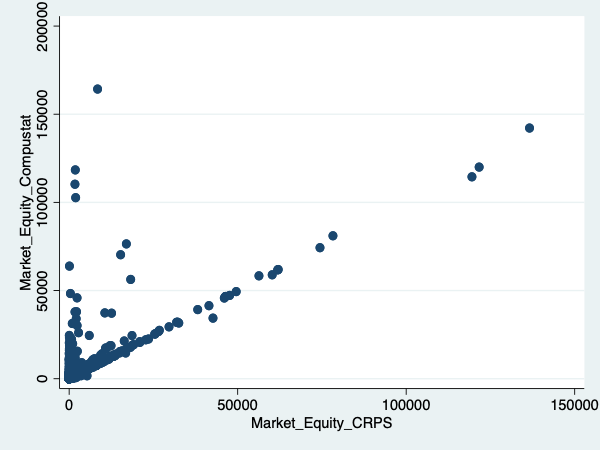
\includegraphics[scale=0.5]{m_equity_scatter}

\begin{tabular}{lc} \hline
 & (1) \\
VARIABLES & Market\_Equity\_Compustat \\ \hline
 &  \\
Market\_Equity\_CRPS & 1.050*** \\
 & (0.00701) \\
Constant & 108.4*** \\
 & (19.05) \\
 &  \\
Observations & 16,263 \\
 R-squared & 0.580 \\ \hline
\multicolumn{2}{c}{ Standard errors in parentheses} \\
\multicolumn{2}{c}{ *** p$<$0.01, ** p$<$0.05, * p$<$0.1} \\
\end{tabular}


\section{Question 5}

\begin{tabular}{lcc} \hline
 & (1) & (2) \\
VARIABLES & b\_lev\_tr & m\_lev\_tr \\ \hline
 &  &  \\
zee\_i\_b\_lev & 0.248*** &  \\
 & (0.00960) &  \\
zee\_l\_sales\_tr & 0.0203*** & 0.0336*** \\
 & (0.00173) & (0.00204) \\
zee\_m\_b\_tr & -0.0147*** & -0.0707*** \\
 & (0.00134) & (0.00165) \\
zee\_profit\_tr & -0.0342*** & -0.0544*** \\
 & (0.00147) & (0.00158) \\
zee\_tang\_tr & 0.0207*** & 0.0168*** \\
 & (0.00176) & (0.00201) \\
zee\_ind\_b\_lev & 0.0412*** & 0.0477*** \\
 & (0.00170) & (0.00176) \\
roa\_vol & -0.115*** & -0.154*** \\
 & (0.0126) & (0.0177) \\
pays\_dv & -0.0442*** & -0.0647*** \\
 & (0.00305) & (0.00362) \\
zee\_i\_m\_lev &  & 0.0864*** \\
 &  & (0.00238) \\
Constant & 0.284*** & 0.328*** \\
 & (0.00254) & (0.00306) \\
 &  &  \\
Observations & 56,970 & 51,313 \\
 R-squared & 0.370 & 0.492 \\ \hline
\multicolumn{3}{c}{ Robust standard errors in parentheses} \\
\multicolumn{3}{c}{ *** p$<$0.01, ** p$<$0.05, * p$<$0.1} \\
\end{tabular}


\end{document}

